% !TeX encoding = UTF-8
% !TeX TS-program = latexmk
% Mathematical Programming: An Introduction to Optimization
% Reconstructed from source PDF pages 1--80 for the 2026--2027 academic year.
% Instructor metadata has been replaced with the user-confirmed information.
% Course-administration details that were not confirmed (assessment weights,
% contact hours, e-mail addresses, and former acknowledgments) are not copied.
%
% Extracted image map:
%   source p.005 -> figures/mp-2026/p005-optimization-manufacturing.jpg
%   source p.006 -> figures/mp-2026/p006-optimization-transportation.jpg
%   source p.068 -> figures/mp-2026/p068-hulls-example.jpg
%   source p.070 -> figures/mp-2026/p070-affine-translate.jpg
%   source p.071 -> figures/mp-2026/p071-hyperplane-halfspaces.jpg
%   source p.072 -> figures/mp-2026/p072-convex-polytope.jpg
%   source p.073 -> figures/mp-2026/p073-simplex-examples.jpg
%   source p.074 -> figures/mp-2026/p074-extreme-points.jpg
%   source p.078 -> figures/mp-2026/p078-unbounded-polyhedron.jpg
%   source p.078 -> figures/mp-2026/p078-bounded-polytope.jpg
%   source p.080 -> figures/mp-2026/p080-finite-basis-decomposition.jpg

\PassOptionsToPackage{cmyk}{xcolor}
\documentclass[
  aspectratio=169,
  hyperref,
  UTF8,
  CJK
]{beamer}

% Use TeX Live fonts rather than host-OS fonts so the deck is portable.
\makeatletter
\newcommand{\beamer@scu@fontextend}{%
  \setsansfont{Latin Modern Sans}%
  \setmonofont{Latin Modern Mono}%
}
\makeatother

\usetheme[
  ColorDisplay=JXred,
  BlockDisplay=followtheme,
  CodeTheme=listing,
  LanguageMode=en,
  Miniframes=follow,
  NavigationTool=1-2-3,
  FontTheme=Custom,
  MathFont=LM,
  BIBMode=none,
  ContentMuticols=false,
  Background=SCU-Full
]{scu}

\usepackage{array}
\usepackage{booktabs}
\usepackage{mathtools}
\usepackage{multirow}
\usepackage{tabularx}

\newcommand{\R}{\mathbb{R}}
\newcommand{\Lin}{\mathcal{L}}
\newcommand{\Aff}{\mathcal{A}}
\newcommand{\Cone}{\mathcal{C}}
\newcommand{\Conv}{\mathcal{X}}
\newcommand{\trans}{\mathsf{T}}
\newcommand{\vect}[1]{\boldsymbol{#1}}

\title[Mathematical Programming]{Mathematical Programming}
\subtitle{An Introduction to Optimization}
\author[Changxi Wang]{Changxi Wang}
\institute{Sichuan University-Pittsburgh Institute}
\date{2026--2027 Academic Year}

% The theme inserts an outline before every subsection by default.  Disable
% those extra pages so the reconstructed deck keeps a one-to-one mapping with
% source PDF pages 1--80 (automatic title page + 79 content frames).
\AtBeginSubsection[]{}

\begin{document}

% Source PDF page 001 is generated automatically by the SCU title-page theme.

\section{Course Orientation}
\subsection{Scope and Motivation}

% Source PDF page 002
\begin{frame}{Course Scope and References}
  \begin{columns}[T,onlytextwidth]
    \begin{column}{0.51\textwidth}
      \structure{Course scope}
      \begin{itemize}
        \item Mathematical programming models and terminology
        \item Linear-algebra foundations for optimization
        \item Affine and convex geometry
        \item Linear programming and polyhedral structure
      \end{itemize}
    \end{column}
    \begin{column}{0.45\textwidth}
      \structure{Primary references}
      \begin{itemize}
        \item Melvyn W. Jeter, \emph{Mathematical Programming: An Introduction to Optimization}
        \item Stephen Boyd and Lieven Vandenberghe, \emph{Convex Optimization}
      \end{itemize}
      \vspace{0.5em}
      \alert{Instructor: Changxi Wang}
    \end{column}
  \end{columns}
\end{frame}

% Source PDF page 003; former-instructor acknowledgments replaced.
\begin{frame}{Learning Objectives}
  By the end of this unit, students should be able to:
  \begin{itemize}
    \item translate a verbal decision problem into variables, objectives, and constraints;
    \item distinguish linear, nonlinear, continuous, and discrete models;
    \item use linear-algebra and topology concepts in optimization arguments;
    \item characterize affine sets, convex sets, polyhedra, and polytopes;
    \item explain why linear-program feasible regions are convex.
  \end{itemize}
\end{frame}

% Source PDF page 004
\begin{frame}{Optimization Turns Decisions into Mathematical Models}
  \begin{itemize}
    \item This course assumes prior study of linear algebra, calculus, and multivariable calculus.
    \item Optimization selects the best feasible decision according to a stated objective.
    \item Representative applications include:
      \begin{itemize}
        \item economic analysis and management;
        \item production planning and logistics;
        \item engineering design and resource allocation;
        \item scheduling, networks, and operations research.
      \end{itemize}
  \end{itemize}
\end{frame}

% Source PDF page 005
\begin{frame}{Optimization Coordinates Production Decisions}
  \begin{columns}[T,onlytextwidth]
    \begin{column}{0.36\textwidth}
      \begin{itemize}
        \item production quantity;
        \item production speed;
        \item inventory and delivery timing;
        \item allocation of limited resources.
      \end{itemize}
      \vspace{0.5em}
      A model makes the trade-offs explicit and testable.
    \end{column}
    \begin{column}{0.60\textwidth}
      \centering
      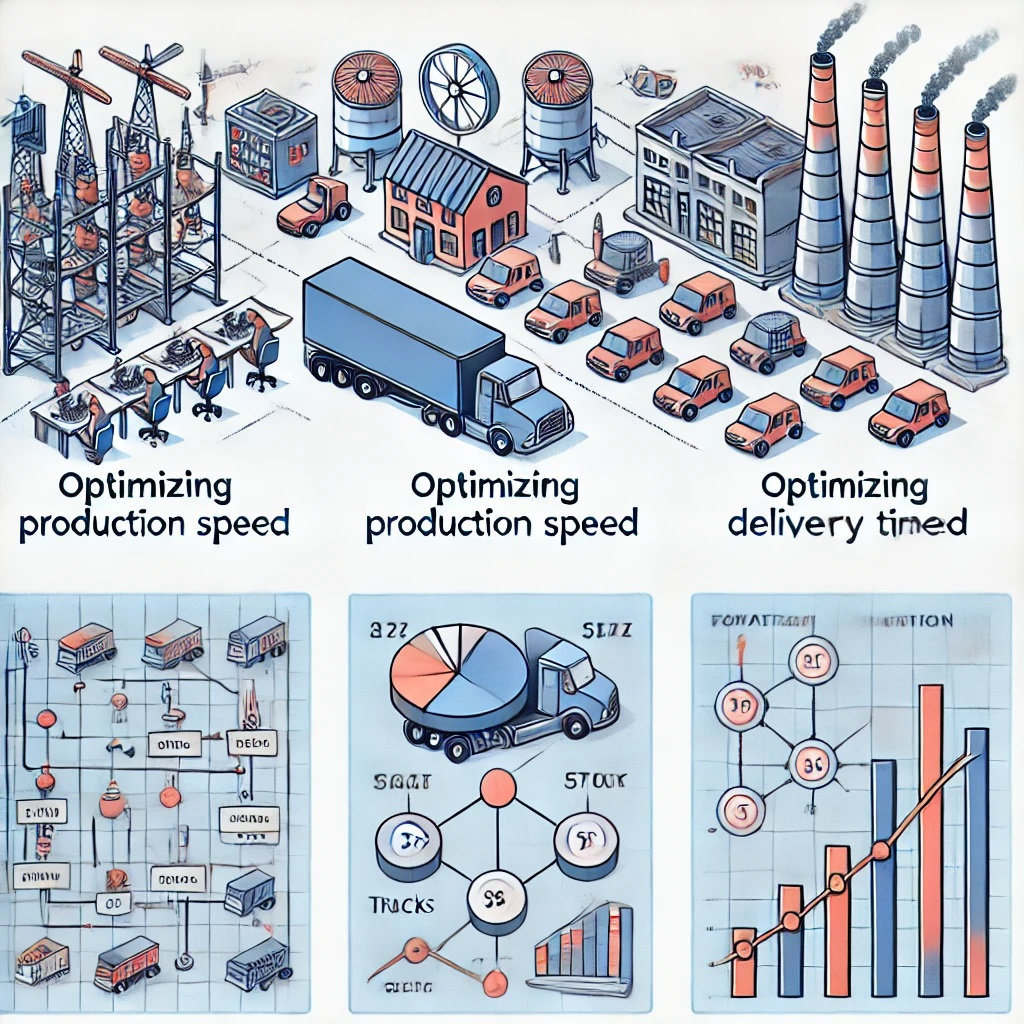
\includegraphics[width=\linewidth,height=0.67\textheight,keepaspectratio]{figures/mp-2026/p005-optimization-manufacturing.jpg}
    \end{column}
  \end{columns}
\end{frame}

% Source PDF page 006
\begin{frame}{Optimization Supports Transportation and Logistics}
  \begin{columns}[T,onlytextwidth]
    \begin{column}{0.38\textwidth}
      \begin{itemize}
        \item vehicle routing;
        \item public-transport planning;
        \item delivery-time control;
        \item network design;
        \item capacity allocation.
      \end{itemize}
    \end{column}
    \begin{column}{0.58\textwidth}
      \centering
      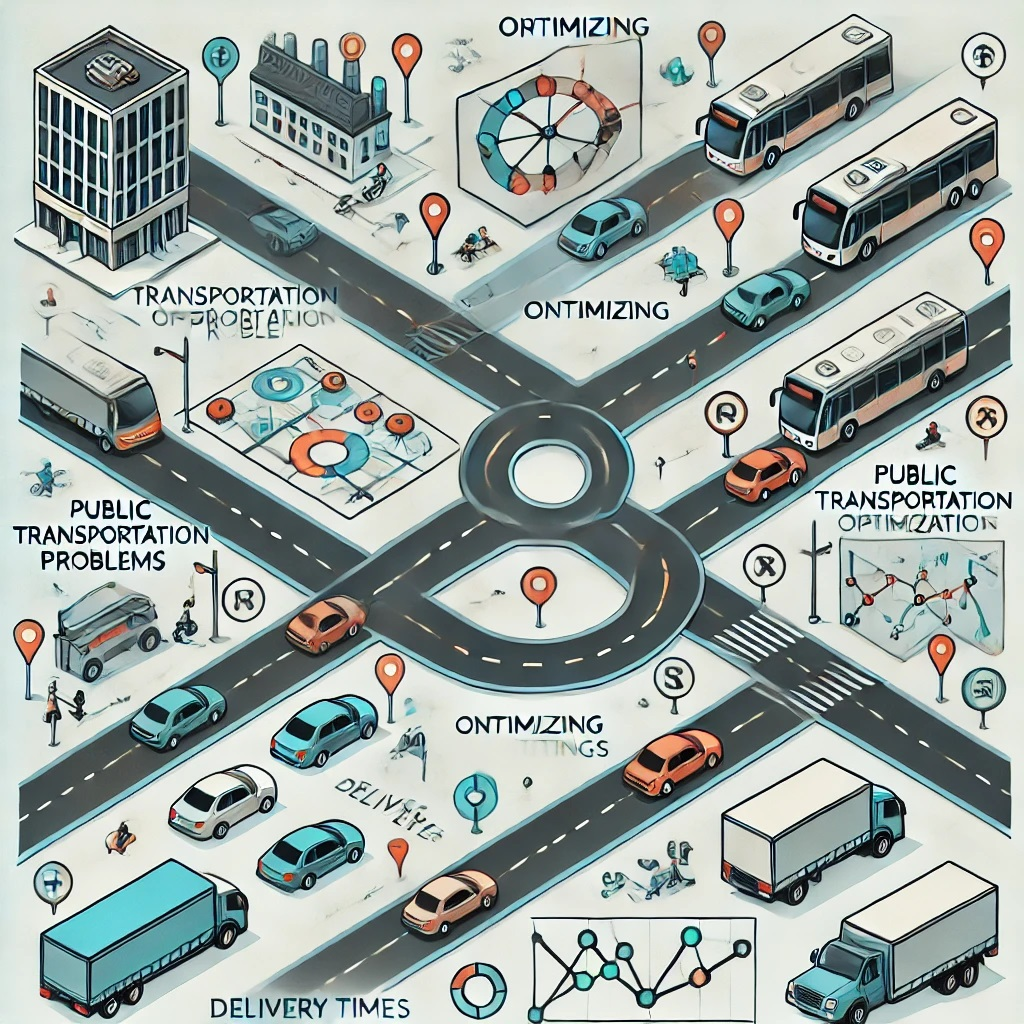
\includegraphics[width=\linewidth,height=0.67\textheight,keepaspectratio]{figures/mp-2026/p006-optimization-transportation.jpg}
    \end{column}
  \end{columns}
\end{frame}

\section{Mathematical Programming Models}
\subsection{Basic Formulations}

% Source PDF page 007
\begin{frame}{A Mathematical Program Has an Objective and a Feasible Set}
  \begin{block}{Generic formulation}
    \begin{equation*}
      \min_{\vect{x}\in\Omega} f(\vect{x})
      \qquad\text{or}\qquad
      \max_{\vect{x}\in\Omega} f(\vect{x}),
      \quad \vect{x}=(x_1,\ldots,x_n)^{\trans}.
    \end{equation*}
  \end{block}
  \begin{itemize}
    \item $f:\R^n\to\R$ is the objective (or cost) function.
    \item $\Omega\subseteq\R^n$ is the feasible set.
    \item The problem is \alert{unconstrained} when $\Omega=\R^n$.
    \item It is \alert{constrained} when feasibility restricts the decision vector.
  \end{itemize}
\end{frame}

% Source PDF page 008
\begin{frame}{A Linear Program Uses Linear Objectives and Constraints}
  \begin{itemize}
    \item Linear objective:
      \begin{equation*}
        f(\vect{x})=c_1x_1+\cdots+c_nx_n=\vect{c}^{\trans}\vect{x}.
      \end{equation*}
    \item Linear equality: $a_1x_1+\cdots+a_nx_n=b$.
    \item Linear inequality: $a_1x_1+\cdots+a_nx_n\le b$ or $\ge b$.
    \item If the objective or any constraint is nonlinear, the model is a nonlinear program.
  \end{itemize}
  \begin{alertblock}{Key distinction}
    Linearity concerns the mathematical expressions, not the application domain.
  \end{alertblock}
\end{frame}

\subsection{Canonical Examples}

% Source PDF page 009
\begin{frame}{Example 1: Production Planning Starts from Resource Data}
  A manufacturer produces products $P_1,\ldots,P_n$ using raw materials $M_1,\ldots,M_m$.
  \begin{center}
    \begin{tabular}{c cccc}
      \toprule
       & $P_1$ & $P_2$ & $\cdots$ & $P_n$ \\
      \midrule
      $M_1$ & $a_{11}$ & $a_{12}$ & $\cdots$ & $a_{1n}$ \\
      $M_2$ & $a_{21}$ & $a_{22}$ & $\cdots$ & $a_{2n}$ \\
      $\vdots$ & $\vdots$ & $\vdots$ & $\ddots$ & $\vdots$ \\
      $M_m$ & $a_{m1}$ & $a_{m2}$ & $\cdots$ & $a_{mn}$ \\
      \bottomrule
    \end{tabular}
  \end{center}
  \begin{itemize}
    \item $b_i$: available units of material $M_i$;
    \item $c_j$: revenue per unit of product $P_j$;
    \item goal: maximize total daily revenue.
  \end{itemize}
\end{frame}

% Source PDF page 010
\begin{frame}{Example 1: Variables Connect Production to Revenue and Usage}
  \begin{itemize}
    \item Decision variable: $x_j=$ number of units of product $P_j$ produced.
    \item Total revenue:
      \begin{equation*}
        c_1x_1+\cdots+c_nx_n=\sum_{j=1}^{n}c_jx_j.
      \end{equation*}
    \item Material $M_i$ consumed:
      \begin{equation*}
        a_{i1}x_1+\cdots+a_{in}x_n=\sum_{j=1}^{n}a_{ij}x_j.
      \end{equation*}
    \item Capacity requirement: $\sum_{j=1}^{n}a_{ij}x_j\le b_i$ for every $i$.
  \end{itemize}
\end{frame}

% Source PDF page 011
\begin{frame}{Example 1: The Production Model Is a Linear Program}
  \begin{equation*}
    \begin{aligned}
      \max_{\vect{x}}\quad & \sum_{j=1}^{n}c_jx_j \\
      \text{subject to}\quad
        & \sum_{j=1}^{n}a_{ij}x_j\le b_i, && i=1,\ldots,m,\\
        & x_j\ge 0, && j=1,\ldots,n.
    \end{aligned}
  \end{equation*}
  In matrix form:
  \begin{equation*}
    \max_{\vect{x}\ge\vect{0}}\ \vect{c}^{\trans}\vect{x}
    \quad\text{subject to}\quad A\vect{x}\le\vect{b}.
  \end{equation*}
\end{frame}

% Source PDF page 012
\begin{frame}{Variable Domains and Slack Variables Change the Model Form}
  \begin{itemize}
    \item A \structure{continuous variable} may take any real value in its allowed interval.
    \item A \structure{discrete variable} takes values from a discrete set, often $\mathbb{Z}$ or $\{0,1\}$.
    \item A \structure{slack variable} converts a $\le$ inequality to an equality:
      \begin{equation*}
        a_{11}x_1+\cdots+a_{1n}x_n\le b_1
        \iff
        a_{11}x_1+\cdots+a_{1n}x_n+s_1=b_1,\qquad s_1\ge0.
      \end{equation*}
    \item A slack variable has objective coefficient zero unless the model assigns it a separate cost.
  \end{itemize}
\end{frame}

% Source PDF page 013
\begin{frame}{Slack Variables Produce Equality Standard Form}
  \small
  \begin{equation*}
    \begin{aligned}
      \max\quad & \sum_{j=1}^{n}c_jx_j+\sum_{i=1}^{m}0\,s_i \\
      \text{subject to}\quad
        & \sum_{j=1}^{n}a_{ij}x_j+s_i=b_i, && i=1,\ldots,m,\\
        & x_j\ge0, && j=1,\ldots,n,\\
        & s_i\ge0, && i=1,\ldots,m.
    \end{aligned}
  \end{equation*}
  With $\vect{s}=\vect{b}-A\vect{x}$, the equality form is feasible exactly when the original inequalities are feasible.
\end{frame}

% Source PDF page 014
\begin{frame}{Example 2: Assignment Uses a Productivity Matrix}
  Four salespeople must be assigned to four sales districts.
  \begin{center}
    \begin{tabular}{c rrrr}
      \toprule
       & $D_1$ & $D_2$ & $D_3$ & $D_4$ \\
      \midrule
      $S_1$ & 5 & 10 & 8 & 2 \\
      $S_2$ & 3 & 4 & 2 & 6 \\
      $S_3$ & 9 & 5 & 4 & 5 \\
      $S_4$ & 5 & 5 & 6 & 4 \\
      \bottomrule
    \end{tabular}
  \end{center}
  The goal is to choose a one-to-one assignment that maximizes total productivity.
\end{frame}

% Source PDF page 015
\begin{frame}{Example 2: Binary Variables Encode an Assignment}
  Define
  \begin{equation*}
    x_{ij}=\begin{cases}
      1, & \text{if salesperson }S_i\text{ is assigned to district }D_j,\\
      0, & \text{otherwise.}
    \end{cases}
  \end{equation*}
  If $r_{ij}$ is the productivity rating, the total value is
  \begin{equation*}
    \sum_{i=1}^{4}\sum_{j=1}^{4}r_{ij}x_{ij}.
  \end{equation*}
  One-to-one assignment requires
  \begin{equation*}
    \sum_{j=1}^{4}x_{ij}=1\quad\forall i,
    \qquad
    \sum_{i=1}^{4}x_{ij}=1\quad\forall j.
  \end{equation*}
\end{frame}

% Source PDF page 016; binary domain corrected from the source relaxation.
\begin{frame}{Example 2: Compact Assignment Formulation}
  \begin{equation*}
    \begin{aligned}
      \max_{\vect{x}}\quad & \sum_{i=1}^{4}\sum_{j=1}^{4}r_{ij}x_{ij} \\
      \text{subject to}\quad
        & \sum_{j=1}^{4}x_{ij}=1, && i=1,\ldots,4,\\
        & \sum_{i=1}^{4}x_{ij}=1, && j=1,\ldots,4,\\
        & x_{ij}\in\{0,1\}, && i,j=1,\ldots,4.
    \end{aligned}
  \end{equation*}
  \begin{alertblock}{Integrality}
    For the assignment constraint matrix, the LP relaxation also has integral extreme points; the binary model states the intended decisions explicitly.
  \end{alertblock}
\end{frame}

% Source PDF page 017
\begin{frame}{Example 3: Production-Line Assignment}
  Three production lines can make flour brands A and B. Entries are ten-pound sacks per day.
  \begin{center}
    \begin{tabular}{c rrr}
      \toprule
       & $L_1$ & $L_2$ & $L_3$ \\
      \midrule
      A & 15000 & 10000 & 12000 \\
      B & 12000 & 13500 & 14500 \\
      \bottomrule
    \end{tabular}
  \end{center}
  \begin{block}{Decision question}
    Assign each line to exactly one brand to maximize total daily output.
  \end{block}
\end{frame}

% Source PDF page 018
\begin{frame}{Example 3: Two Binary Indicators per Production Line}
  For each line $L_i$, define
  \begin{equation*}
    x_i=\begin{cases}1,&L_i\text{ makes A},\\0,&\text{otherwise,}\end{cases}
    \qquad
    w_i=\begin{cases}1,&L_i\text{ makes B},\\0,&\text{otherwise.}\end{cases}
  \end{equation*}
  Complementarity can be written as
  \begin{equation*}
    x_iw_i=0,\qquad i=1,2,3.
  \end{equation*}
  Together with $x_i,w_i\ge0$, this prevents simultaneous assignment to both brands, but it does not yet force a line to be used.
\end{frame}

% Source PDF page 019
\begin{frame}{Example 3: Exact Assignment Makes Complementarity Redundant}
  Requiring every line to make exactly one brand gives
  \begin{equation*}
    x_i+w_i=1,\qquad i=1,2,3,
  \end{equation*}
  with $x_i,w_i\in\{0,1\}$.
  \begin{itemize}
    \item These constraints already imply $x_iw_i=0$.
    \item The single aggregate condition $\sum_{i=1}^{3}x_iw_i=0$ is equivalent only under nonnegativity.
    \item The binary linear formulation is simpler than retaining a nonlinear complementarity constraint.
  \end{itemize}
\end{frame}

% Source PDF page 020
\begin{frame}{Example 3: A Complementarity Formulation Is Nonlinear}
  \small
  \begin{equation*}
    \begin{aligned}
      \max_{\vect{x},\vect{w}}\quad
        &15000x_1+10000x_2+12000x_3\\
        &+12000w_1+13500w_2+14500w_3\\
      \text{subject to}\quad
        &x_i+w_i=1, && i=1,2,3,\\
        &\sum_{i=1}^{3}x_iw_i=0,\\
        &0\le x_i,w_i\le1, && i=1,2,3.
    \end{aligned}
  \end{equation*}
  The product terms make this formulation nonlinear. With binary variables, the product constraint can be removed.
\end{frame}

% Source PDF page 021
\begin{frame}{Example 4: Quadratic Programming Adds Pairwise Terms}
  A quadratic program may take the form
  \begin{equation*}
    \begin{aligned}
      \max_{\vect{x}}\quad
        &\vect{c}^{\trans}\vect{x}+\vect{x}^{\trans}B\vect{x}\\
      \text{subject to}\quad
        &A\vect{x}=\vect{b},\\
        &\vect{x}\ge\vect{0}.
    \end{aligned}
  \end{equation*}
  Equivalently,
  \begin{equation*}
    \vect{x}^{\trans}B\vect{x}=\sum_{i=1}^{n}\sum_{j=1}^{n}b_{ij}x_ix_j.
  \end{equation*}
  Convexity or concavity depends on the quadratic matrix and on whether the problem minimizes or maximizes.
\end{frame}

% Source PDF page 022
\begin{frame}{Example 4: Portfolio Selection Trades Return for Risk}
  \begin{equation*}
    \begin{aligned}
      \max_{\vect{x}}\quad
        & \vect{c}^{\trans}\vect{x}-\vect{x}^{\trans}B\vect{x}\\
      \text{subject to}\quad
        & \vect{1}^{\trans}\vect{x}=1,\\
        & \vect{x}\ge\vect{0}.
    \end{aligned}
  \end{equation*}
  \begin{itemize}
    \item $x_i$: fraction invested in asset $i$;
    \item $c_i$: expected return of asset $i$;
    \item $\vect{x}^{\trans}B\vect{x}$: quadratic risk measure;
    \item the minus sign penalizes risk while rewarding expected return.
  \end{itemize}
\end{frame}

\subsection{Solutions, Topology, and Sensitivity}

% Source PDF page 023
\begin{frame}{Neighborhoods Formalize What ``Local'' Means}
  For $\vect{x},\bar{\vect{x}}\in\R^n$, the Euclidean distance is
  \begin{equation*}
    \|\vect{x}-\bar{\vect{x}}\|_2
      =\sqrt{\sum_{i=1}^{n}(x_i-\bar{x}_i)^2}.
  \end{equation*}
  The open $\varepsilon$-neighborhood of $\bar{\vect{x}}$ is
  \begin{equation*}
    N_{\varepsilon}(\bar{\vect{x}})
      =\{\vect{x}\in\R^n:\|\vect{x}-\bar{\vect{x}}\|_2<\varepsilon\},
      \qquad\varepsilon>0.
  \end{equation*}
  Local optimality compares feasible points only inside such a neighborhood.
\end{frame}

% Source PDF page 024; strict/global definitions corrected.
\begin{frame}{Local and Global Minima Differ by Comparison Set}
  Let $\bar{\vect{x}}\in\Omega$.
  \begin{itemize}
    \item \structure{Local minimum}: there exists $\varepsilon>0$ such that
      \begin{equation*}
        f(\bar{\vect{x}})\le f(\vect{x})
        \quad\forall\vect{x}\in\Omega\cap N_{\varepsilon}(\bar{\vect{x}}).
      \end{equation*}
    \item \structure{Strict local minimum}: replace $\le$ by $<$ for every feasible $\vect{x}\ne\bar{\vect{x}}$ in that neighborhood.
    \item \structure{Global minimum}: $f(\bar{\vect{x}})\le f(\vect{x})$ for all $\vect{x}\in\Omega$.
    \item \structure{Strict global minimum}: $f(\bar{\vect{x}})<f(\vect{x})$ for all $\vect{x}\in\Omega\setminus\{\bar{\vect{x}}\}$.
  \end{itemize}
\end{frame}

% Source PDF page 025
\begin{frame}{Interior, Open Sets, and Exterior}
  \begin{align*}
    \operatorname{Int}(\Omega)
      &=\{\vect{x}\in\Omega:\exists\varepsilon>0,
          N_{\varepsilon}(\vect{x})\subseteq\Omega\},\\
    \operatorname{Ext}(\Omega)
      &=\{\vect{x}\in\R^n:\exists\varepsilon>0,
          N_{\varepsilon}(\vect{x})\subseteq\R^n\setminus\Omega\}.
  \end{align*}
  \begin{itemize}
    \item $\Omega$ is open when $\Omega=\operatorname{Int}(\Omega)$.
    \item Every point of an open set has a sufficiently small neighborhood contained in the set.
    \item The exterior is the interior of the complement.
  \end{itemize}
\end{frame}

% Source PDF page 026
\begin{frame}{Boundary and Accumulation Points Describe Set Limits}
  \begin{itemize}
    \item $\vect{x}$ is a \structure{boundary point} of $\Omega$ when every neighborhood intersects both $\Omega$ and $\R^n\setminus\Omega$.
    \item The boundary is
      \begin{equation*}
        \partial\Omega=\overline{\Omega}\setminus\operatorname{Int}(\Omega).
      \end{equation*}
    \item $\Omega$ is closed when it contains all of its boundary points, equivalently $\overline{\Omega}=\Omega$.
    \item $\vect{x}$ is an \structure{accumulation point} if
      \begin{equation*}
        \forall\varepsilon>0,\quad
        \bigl(N_{\varepsilon}(\vect{x})\setminus\{\vect{x}\}\bigr)\cap\Omega\ne\varnothing.
      \end{equation*}
  \end{itemize}
\end{frame}

% Source PDF page 027
\begin{frame}{Sensitivity Analysis Reuses Structure after Data Change}
  Model data are estimates or measurements and may change over time.
  \vspace{1em}
  \begin{columns}[c,onlytextwidth]
    \begin{column}{0.38\textwidth}
      \begin{block}{Existing problem}
        Known data, feasible set, and optimal solution
      \end{block}
    \end{column}
    \begin{column}{0.16\textwidth}
      \centering
      $\Longrightarrow$
    \end{column}
    \begin{column}{0.38\textwidth}
      \begin{block}{Modified problem}
        Updated data and a revised optimal solution
      \end{block}
    \end{column}
  \end{columns}
  \vspace{1em}
  Post-optimal analysis asks whether the original solution or factorization can be updated without solving from scratch.
\end{frame}

% Source PDF page 028
\begin{frame}{Example 5: Transportation Balances Supply and Demand}
  \begin{itemize}
    \item Products are stored at $m$ origins and sold at $n$ outlets.
    \item $c_{ij}$ is the unit shipping cost from origin $i$ to outlet $j$.
    \item Origin $i$ has $s_i$ units available.
    \item Outlet $j$ requires exactly $d_j$ units.
    \item Decision variable $x_{ij}$ is the quantity shipped from $i$ to $j$.
  \end{itemize}
  \begin{block}{Goal}
    Meet all outlet demands at minimum total shipping cost without exceeding any origin's supply.
  \end{block}
\end{frame}

% Source PDF page 029
\begin{frame}{Example 5: Transportation Model}
  \begin{equation*}
    \begin{aligned}
      \min_{\vect{x}}\quad
        &\sum_{i=1}^{m}\sum_{j=1}^{n}c_{ij}x_{ij}\\
      \text{subject to}\quad
        &\sum_{j=1}^{n}x_{ij}\le s_i, && i=1,\ldots,m,\\
        &\sum_{i=1}^{m}x_{ij}=d_j, && j=1,\ldots,n,\\
        &x_{ij}\ge0, && i=1,\ldots,m,\ j=1,\ldots,n.
    \end{aligned}
  \end{equation*}
  Feasibility requires total available supply to be at least total demand.
\end{frame}

% Source PDF page 030
\begin{frame}{Parametric Programming Models Demand Growth}
  Suppose outlet $j$ has current demand $d_j$ and daily growth $\bar d_j$. After $t\ge0$ days:
  \begin{equation*}
    \begin{aligned}
      \min_{\vect{x}}\quad
        &\sum_{i=1}^{m}\sum_{j=1}^{n}c_{ij}x_{ij}\\
      \text{subject to}\quad
        &\sum_{j=1}^{n}x_{ij}\le s_i, && i=1,\ldots,m,\\
        &\sum_{i=1}^{m}x_{ij}=d_j+t\bar d_j, && j=1,\ldots,n,\\
        &x_{ij}\ge0.
    \end{aligned}
  \end{equation*}
  The parameter $t$ changes both feasibility and the optimal shipping plan.
\end{frame}

% Source PDF page 031; wording refined to avoid overclaiming redundancy.
\begin{frame}{Model Stability Measures Sensitivity to Perturbations}
  \begin{itemize}
    \item A \structure{stable} model exhibits small changes in the optimizer and optimal value under small data perturbations.
    \item An \structure{unstable} or ill-conditioned model can exhibit large changes under small perturbations.
    \item Near-dependent or redundant constraints may amplify numerical sensitivity.
  \end{itemize}
  \begin{equation*}
    \sum_{i=1}^{m}\lambda_i g_i(\vect{x})
      =\sum_{i=1}^{m}\lambda_i b_i
    \quad\longrightarrow\quad
    \sum_{i=1}^{m}\lambda_i g_i(\vect{x})
      =\varepsilon+\sum_{i=1}^{m}\lambda_i b_i.
  \end{equation*}
  A tiny inconsistent perturbation $\varepsilon\ne0$ can destroy feasibility when one constraint is an exact linear combination of others.
\end{frame}

\section{Linear Algebra Review}
\subsection{Matrices and Vectors}

% Source PDF page 032
\begin{frame}{Matrices Organize Linear Maps and Constraints}
  \begin{equation*}
    A=\begin{bmatrix}
      a_{11}&a_{12}&\cdots&a_{1n}\\
      a_{21}&a_{22}&\cdots&a_{2n}\\
      \vdots&\vdots&\ddots&\vdots\\
      a_{m1}&a_{m2}&\cdots&a_{mn}
    \end{bmatrix}
    =[a_{ij}]\in\R^{m\times n}.
  \end{equation*}
  \begin{itemize}
    \item $a_{ij}$ is the entry in row $i$ and column $j$.
    \item $\R^{m\times n}$ is the set of all real $m\times n$ matrices.
    \item In optimization, rows often represent constraints and columns represent variables.
  \end{itemize}
\end{frame}

% Source PDF page 033
\begin{frame}{Transposition Exchanges Rows and Columns}
  If $A\in\R^{m\times n}$, then $A^{\trans}\in\R^{n\times m}$ and
  \begin{equation*}
    A^{\trans}=\begin{bmatrix}
      a_{11}&a_{21}&\cdots&a_{m1}\\
      a_{12}&a_{22}&\cdots&a_{m2}\\
      \vdots&\vdots&\ddots&\vdots\\
      a_{1n}&a_{2n}&\cdots&a_{mn}
    \end{bmatrix},
    \qquad (A^{\trans})_{ij}=A_{ji}.
  \end{equation*}
  Useful identities:
  \begin{equation*}
    (A+B)^{\trans}=A^{\trans}+B^{\trans},
    \qquad (AB)^{\trans}=B^{\trans}A^{\trans}.
  \end{equation*}
\end{frame}

% Source PDF page 034
\begin{frame}{Column and Row Vectors Have Different Shapes}
  \begin{align*}
    \vect{x}
      &=\begin{bmatrix}x_1&\cdots&x_m\end{bmatrix}^{\trans}
        \in\R^{m\times1},\\
    \vect{y}^{\trans}
      &=\begin{bmatrix}y_1&\cdots&y_n\end{bmatrix}
        \in\R^{1\times n}.
  \end{align*}
  \begin{itemize}
    \item Scalars are real or complex numbers.
    \item $\R^m$ denotes Euclidean $m$-space and is usually identified with $\R^{m\times1}$.
    \item Optimization decision variables are conventionally written as column vectors.
  \end{itemize}
\end{frame}

% Source PDF page 035
\begin{frame}{Vector Addition and Scalar Multiplication Are Componentwise}
  For $\vect{x},\vect{y}\in\R^n$ and $\alpha\in\R$,
  \begin{align*}
    \vect{x}+\vect{y}
      &=[x_1+y_1,\ldots,x_n+y_n]^{\trans},\\
    \alpha\vect{x}
      &=[\alpha x_1,\ldots,\alpha x_n]^{\trans}.
  \end{align*}
  These operations satisfy closure, associativity, commutativity of addition, distributivity, and the usual identity and inverse properties.
\end{frame}

% Source PDF page 036; inner-product index and norm corrected.
\begin{frame}{The Inner Product Induces the Euclidean Norm}
  \begin{equation*}
    \langle\vect{x},\vect{y}\rangle
      =\vect{x}^{\trans}\vect{y}
      =\sum_{i=1}^{n}x_i y_i.
  \end{equation*}
  \begin{itemize}
    \item Symmetry: $\langle\vect{x},\vect{y}\rangle=\langle\vect{y},\vect{x}\rangle$.
    \item Linearity: $\langle\alpha\vect{x}+\beta\vect{y},\vect{z}\rangle=\alpha\langle\vect{x},\vect{z}\rangle+\beta\langle\vect{y},\vect{z}\rangle$.
    \item Positive definiteness: $\langle\vect{x},\vect{x}\rangle\ge0$, with equality iff $\vect{x}=\vect{0}$.
    \item Euclidean norm:
      \begin{equation*}
        \|\vect{x}\|_2=\sqrt{\langle\vect{x},\vect{x}\rangle}
        =\sqrt{\vect{x}^{\trans}\vect{x}}.
      \end{equation*}
  \end{itemize}
\end{frame}

\subsection{Subspaces, Span, and Rank}

% Source PDF page 037
\begin{frame}{A Subspace Is Closed under Linear Combinations}
  A nonempty set $S\subseteq\R^n$ is a subspace if
  \begin{equation*}
    \vect{x},\vect{y}\in S, \alpha,\beta\in\R
    \quad\Longrightarrow\quad
    \alpha\vect{x}+\beta\vect{y}\in S.
  \end{equation*}
  For $B\subseteq\R^n$, its linear span is
  \begin{equation*}
    \Lin(B)=
    \left\{\sum_{i=1}^{k}\alpha_i\vect{x}_i:
      \alpha_i\in\R,\ \vect{x}_i\in B,\ k\in\mathbb{N}\right\}.
  \end{equation*}
  $\Lin(B)$ collects all finite linear combinations of vectors in $B$.
\end{frame}

% Source PDF page 038
\begin{frame}{Example 5: The Standard Basis Spans $\R^3$}
  Let
  \begin{equation*}
    B_1=\{(1,0,0)^{\trans},(0,1,0)^{\trans},(0,0,1)^{\trans}\}.
  \end{equation*}
  Then
  \begin{align*}
    \Lin(B_1)
      &=\{x_1(1,0,0)^{\trans}+x_2(0,1,0)^{\trans}+x_3(0,0,1)^{\trans}:x_i\in\R\}\\
      &=\{(x_1,x_2,x_3)^{\trans}:x_i\in\R\}
       =\R^3.
  \end{align*}
\end{frame}

% Source PDF page 039
\begin{frame}{Example 6: Two Vectors Span the $x_1$-$x_3$ Plane}
  Let
  \begin{equation*}
    B_2=\{(1,0,0)^{\trans},(1,0,1)^{\trans}\}.
  \end{equation*}
  Then
  \begin{align*}
    \Lin(B_2)
      &=\{x_1(1,0,0)^{\trans}+x_2(1,0,1)^{\trans}:x_1,x_2\in\R\}\\
      &=\{(x_1+x_2,0,x_2)^{\trans}:x_1,x_2\in\R\}\\
      &=\{(u,0,v)^{\trans}:u,v\in\R\}.
  \end{align*}
  Thus $\Lin(B_2)$ is the $x_1$-$x_3$ plane.
\end{frame}

% Source PDF page 040
\begin{frame}{Example 6: Adding a Dependent Vector Does Not Enlarge the Span}
  Let
  \begin{equation*}
    B_3=\{(1,0,0)^{\trans},(1,0,1)^{\trans},(4,0,1)^{\trans}\}.
  \end{equation*}
  Because
  \begin{equation*}
    (4,0,1)^{\trans}=3(1,0,0)^{\trans}+(1,0,1)^{\trans},
  \end{equation*}
  the third vector is already in $\Lin(B_2)$. Therefore
  \begin{equation*}
    \Lin(B_3)=\Lin(B_2)=\{(u,0,v)^{\trans}:u,v\in\R\}.
  \end{equation*}
\end{frame}

% Source PDF page 041
\begin{frame}{The Span Is the Smallest Subspace Containing a Set}
  \begin{itemize}
    \item $\Lin(B)$ is a subspace of $\R^n$.
    \item If $S=\Lin(B)$, then $B$ spans $S$.
    \item Any intersection of subspaces of $\R^n$ is also a subspace.
    \item The span can be characterized by
      \begin{equation*}
        \Lin(B)=\bigcap\{S:S\text{ is a subspace of }\R^n\text{ and }B\subseteq S\}.
      \end{equation*}
  \end{itemize}
  Hence $\Lin(B)$ is the unique smallest subspace containing $B$.
\end{frame}

% Source PDF page 042
\begin{frame}{Example 7: Solve the Constraint to Find a Spanning Set}
  Let
  \begin{equation*}
    S=\{(x_1,x_2,x_3)^{\trans}:x_1+x_2=0\}.
  \end{equation*}
  Since $x_2=-x_1$,
  \begin{align*}
    S
      &=\{(x_1,-x_1,x_3)^{\trans}:x_1,x_3\in\R\}\\
      &=\{x_1(1,-1,0)^{\trans}+x_3(0,0,1)^{\trans}:x_1,x_3\in\R\}\\
      &=\Lin\{(1,-1,0)^{\trans},(0,0,1)^{\trans}\}.
  \end{align*}
  Thus $S$ is a two-dimensional subspace.
\end{frame}

% Source PDF page 043
\begin{frame}{A Basis Is Independent and Spans the Space}
  A set $B$ is linearly dependent if there exist distinct vectors $\vect{x}_1,\ldots,\vect{x}_k\in B$ and scalars, not all zero, such that
  \begin{equation*}
    \alpha_1\vect{x}_1+\cdots+\alpha_k\vect{x}_k=\vect{0}.
  \end{equation*}
  Otherwise $B$ is linearly independent.
  \begin{block}{Basis}
    $B$ is a basis for a subspace $S$ if:
    \begin{enumerate}
      \item $\Lin(B)=S$;
      \item $B$ is linearly independent.
    \end{enumerate}
  \end{block}
\end{frame}

% Source PDF page 044
\begin{frame}{Dimension Counts the Vectors in Any Basis}
  For a finite-dimensional subspace $S$:
  \begin{itemize}
    \item every basis of $S$ has the same number of vectors, denoted $\dim(S)$;
    \item every finite spanning set contains a basis;
    \item every linearly independent set can be extended to a basis;
    \item more than $\dim(S)$ vectors in $S$ must be linearly dependent;
    \item if $S\subseteq T$, then $\dim(S)\le\dim(T)$.
  \end{itemize}
\end{frame}

% Source PDF page 045
\begin{frame}{Rows and Columns Are Vectors in Different Spaces}
  For $A=[a_{ij}]\in\R^{m\times n}$:
  \begin{align*}
    A^{(j)}&=(a_{1j},\ldots,a_{mj})^{\trans}\in\R^m,
      &&\text{the $j$-th column},\\
    A_{(i)}&=(a_{i1},\ldots,a_{in})\in\R^{1\times n},
      &&\text{the $i$-th row}.
  \end{align*}
  The same matrix can therefore be viewed as
  \begin{equation*}
    A=[A^{(1)}\ \cdots\ A^{(n)}]
    \qquad\text{or as a stack of row vectors.}
  \end{equation*}
\end{frame}

% Source PDF page 046
\begin{frame}{Row Rank Equals Column Rank}
  \begin{itemize}
    \item Column space: $\operatorname{col}(A)=\Lin\{A^{(1)},\ldots,A^{(n)}\}\subseteq\R^m$.
    \item Row space: $\operatorname{row}(A)=\Lin\{A_{(1)},\ldots,A_{(m)}\}\subseteq\R^n$.
    \item The fundamental rank theorem gives
      \begin{equation*}
        \operatorname{rank}(A)
          =\dim\operatorname{col}(A)
          =\dim\operatorname{row}(A).
      \end{equation*}
  \end{itemize}
  Rank measures the number of independent directions represented by the matrix.
\end{frame}

\subsection{Matrix Operations and Linear Systems}

% Source PDF page 047
\begin{frame}{Matrix Operations Extend Scalar Arithmetic}
  For conformable matrices:
  \begin{align*}
    A+B&=[a_{ij}+b_{ij}],\\
    \alpha A&=[\alpha a_{ij}],\\
    (AB)_{ij}&=\sum_{\ell=1}^{k}a_{i\ell}b_{\ell j},
      &&A\in\R^{m\times k},\ B\in\R^{k\times n}.
  \end{align*}
  Therefore $AB\in\R^{m\times n}$. In general, matrix multiplication is associative and distributive but not commutative.
\end{frame}

% Source PDF page 048; terminology corrected from ``Dirac function.''
\begin{frame}{The Identity Matrix Uses the Kronecker Delta}
  \begin{equation*}
    I_n=\begin{bmatrix}
      1&0&\cdots&0\\
      0&1&\cdots&0\\
      \vdots&\vdots&\ddots&\vdots\\
      0&0&\cdots&1
    \end{bmatrix}
    =[\delta_{ij}]\in\R^{n\times n},
  \end{equation*}
  where the Kronecker delta is
  \begin{equation*}
    \delta_{ij}=\begin{cases}1,&i=j,\\0,&i\ne j.\end{cases}
  \end{equation*}
  For every conformable matrix $A$, $AI=IA=A$.
\end{frame}

% Source PDF page 049
\begin{frame}{A Submatrix Selects Rows and Columns from a Matrix}
  Consider
  \begin{equation*}
    A=\begin{bmatrix}
      6&1&3&4&0&5\\
      2&1&4&0&0&1\\
      1&0&1&-1&1&0
    \end{bmatrix}.
  \end{equation*}
  Selecting rows $\{2,3\}$ and columns $\{3,4,6\}$ gives
  \begin{equation*}
    B=\begin{bmatrix}
      4&0&1\\
      1&-1&0
    \end{bmatrix}.
  \end{equation*}
  Submatrices support block algebra, factorization, and decomposition arguments.
\end{frame}

% Source PDF page 050
\begin{frame}{Partitioned Matrices Treat Submatrices as Blocks}
  The matrix from the previous slide can be partitioned as
  \begin{equation*}
    A=
    \left[\begin{array}{cc|cc|c|c}
      6&1&3&4&0&5\\
      2&1&4&0&0&1\\ \hline
      1&0&1&-1&1&0
    \end{array}\right]
    =\begin{bmatrix}
      B&D&O&\vect{b}\\
      -\vect{c}_B^{\trans}&-\vect{c}_D^{\trans}&1&0
    \end{bmatrix},
  \end{equation*}
  with
  \begin{equation*}
    B=\begin{bmatrix}6&1\\2&1\end{bmatrix},\quad
    D=\begin{bmatrix}3&4\\4&0\end{bmatrix},\quad
    O=\begin{bmatrix}0\\0\end{bmatrix},\quad
    \vect{b}=\begin{bmatrix}5\\1\end{bmatrix}.
  \end{equation*}
\end{frame}

% Source PDF page 051; lower-right block corrected to EJ+FM.
\begin{frame}{Block Multiplication Follows the Same Conformability Rules}
  Let
  \begin{equation*}
    A=\begin{bmatrix}C&D\\E&F\end{bmatrix},
    \qquad
    B=\begin{bmatrix}G&H&J\\K&L&M\end{bmatrix}.
  \end{equation*}
  Then
  \begin{equation*}
    AB=\begin{bmatrix}
      CG+DK & CH+DL & CJ+DM\\
      EG+FK & EH+FL & EJ+FM
    \end{bmatrix}.
  \end{equation*}
  Each block product must be dimensionally conformable.
\end{frame}

% Source PDF page 052
\begin{frame}{A Nonsingular Matrix Has a Two-Sided Inverse}
  For $A,B\in\R^{n\times n}$,
  \begin{equation*}
    AB=BA=I_n
  \end{equation*}
  means that $A$ is nonsingular and $B=A^{-1}$.
  \begin{itemize}
    \item The inverse, when it exists, is unique.
    \item A matrix without an inverse is singular.
    \item $(AB)^{-1}=B^{-1}A^{-1}$ for nonsingular $A$ and $B$.
  \end{itemize}
\end{frame}

% Source PDF page 053
\begin{frame}{Full Rank Characterizes Nonsingularity}
  For a square matrix $A\in\R^{n\times n}$, the following are equivalent:
  \begin{equation*}
    A\text{ is nonsingular}
    \iff \operatorname{rank}(A)=n
    \iff \text{columns of }A\text{ are independent}.
  \end{equation*}
  Compare
  \begin{equation*}
    \underbrace{\begin{bmatrix}1&1&4\\0&0&0\\0&1&1\end{bmatrix}}_{\text{singular}}
    \qquad
    \underbrace{\begin{bmatrix}1&0&0\\1&1&0\\1&1&1\end{bmatrix}}_{\text{nonsingular}}.
  \end{equation*}
\end{frame}

% Source PDF page 054
\begin{frame}{Elementary Row Operations Preserve the Row Space}
  The three elementary row operations are:
  \begin{enumerate}
    \item scale a row by $\alpha\ne0$;
    \item replace row $i$ by row $i+\alpha$ row $j$;
    \item exchange two rows.
  \end{enumerate}
  To compute an inverse, row reduce the augmented matrix:
  \begin{equation*}
    [A\mid I_n]\ \longrightarrow\ [I_n\mid A^{-1}].
  \end{equation*}
  Failure to obtain $I_n$ on the left means that $A$ is singular.
\end{frame}

% Source PDF page 055
\begin{frame}{A Block-Triangular Matrix Has a Simple Inverse}
  Let $B\in\R^{m\times m}$ be nonsingular. Then
  \begin{equation*}
    \begin{bmatrix}
      B&\vect{0}\\
      -\vect{c}_B^{\trans}&1
    \end{bmatrix}^{-1}
    =
    \begin{bmatrix}
      B^{-1}&\vect{0}\\
      \vect{c}_B^{\trans}B^{-1}&1
    \end{bmatrix}.
  \end{equation*}
  Verification follows by block multiplication:
  \begin{equation*}
    \begin{bmatrix}B^{-1}&0\\\vect{c}_B^{\trans}B^{-1}&1\end{bmatrix}
    \begin{bmatrix}B&0\\-\vect{c}_B^{\trans}&1\end{bmatrix}
    =I_{m+1}.
  \end{equation*}
\end{frame}

% Source PDF page 056
\begin{frame}{The Same Row Operations Extend to a Block System}
  Suppose row operations transform
  \begin{equation*}
    [B\mid I_m]\ \longrightarrow\ [I_m\mid B^{-1}].
  \end{equation*}
  Applying them to the upper block row gives
  \begin{equation*}
    \left[
      \begin{array}{cc|cc}
        B&0&I_m&0\\
        -\vect{c}_B^{\trans}&1&0^{\trans}&1
      \end{array}
    \right]
    \longrightarrow
    \left[
      \begin{array}{cc|cc}
        I_m&0&B^{-1}&0\\
        -\vect{c}_B^{\trans}&1&0^{\trans}&1
      \end{array}
    \right].
  \end{equation*}
  Adding $\vect{c}_B^{\trans}$ times the block row to the last row yields the inverse on the right.
\end{frame}

% Source PDF page 057
\begin{frame}{Example 8: Solve a Linear System}
  Solve $A\vect{x}=\vect{b}$ for
  \begin{equation*}
    A=\begin{bmatrix}
      1&1&-1\\
      -2&1&1\\
      1&1&1
    \end{bmatrix},
    \qquad
    \vect{b}=\begin{bmatrix}1\\2\\0\end{bmatrix}.
  \end{equation*}
  We can row reduce $[A\mid I\mid\vect{b}]$ to obtain both $A^{-1}$ and $\vect{x}=A^{-1}\vect{b}$.
\end{frame}

% Source PDF page 058
\begin{frame}{Example 8: Gauss-Jordan Elimination Gives $A^{-1}$ and $\vect{x}$}
  \small
  Row reduction produces
  \begin{equation*}
    [A\mid I_3\mid\vect{b}]
    \longrightarrow
    [I_3\mid A^{-1}\mid\vect{x}],
  \end{equation*}
  where
  \begin{equation*}
    A^{-1}=\begin{bmatrix}
      0&-\tfrac13&\tfrac13\\
      \tfrac12&\tfrac13&\tfrac16\\
      -\tfrac12&0&\tfrac12
    \end{bmatrix},
    \qquad
    \vect{x}=\begin{bmatrix}-\tfrac23\\[1mm]\tfrac76\\[1mm]-\tfrac12\end{bmatrix}.
  \end{equation*}
  Direct substitution confirms $A\vect{x}=\vect{b}$.
\end{frame}

% Source PDF page 059
\begin{frame}{Elementary Matrices Encode Row Operations}
  \begin{itemize}
    \item The augmented matrix for $A\vect{x}=\vect{b}$ is $[A\mid\vect{b}]$.
    \item Gauss-Jordan elimination transforms it to $[I\mid A^{-1}\vect{b}]$ when $A$ is nonsingular.
    \item Performing a row operation on $I$ produces an elementary matrix $E$.
  \end{itemize}
  For example,
  \begin{equation*}
    E_1=\begin{bmatrix}1&0&0\\2&1&0\\0&0&1\end{bmatrix},
    \qquad
    E_2=\begin{bmatrix}1&0&0\\0&1&0\\-1&0&1\end{bmatrix}.
  \end{equation*}
  Left multiplication $EA$ applies the corresponding row operation to $A$.
\end{frame}

% Source PDF page 060
\begin{frame}{Gaussian Elimination Separates Forward and Backward Steps}
  \begin{itemize}
    \item \structure{Forward elimination}: transform $[A\mid\vect{b}]$ to $[U\mid\bar{\vect{b}}]$, where $U$ is upper triangular.
    \item \structure{Back substitution}: solve the triangular system from the last variable upward.
  \end{itemize}
  Example system:
  \begin{equation*}
    \begin{aligned}
      2x_2-x_3&=8,\\
      x_1+2x_2&=6,\\
      3x_2+4x_3&=12.
    \end{aligned}
  \end{equation*}
\end{frame}

% Source PDF page 061
\begin{frame}{Gaussian Elimination Produces an Upper-Triangular System}
  \small
  \begin{equation*}
    \left[\begin{array}{ccc|c}
      0&2&-1&8\\
      1&2&0&6\\
      0&3&4&12
    \end{array}\right]
    \xrightarrow{R_1\leftrightarrow R_2}
    \left[\begin{array}{ccc|c}
      1&2&0&6\\
      0&2&-1&8\\
      0&3&4&12
    \end{array}\right]
  \end{equation*}
  \begin{equation*}
    \xrightarrow{R_2\leftrightarrow R_3,\ R_3\leftarrow R_3-\frac23R_2}
    \left[\begin{array}{ccc|c}
      1&2&0&6\\
      0&3&4&12\\
      0&0&-\tfrac{11}{3}&0
    \end{array}\right].
  \end{equation*}
  Back substitution gives $x_3=0$, $x_2=4$, and $x_1=-2$.
\end{frame}

% Source PDF page 062; -11/13 corrected to -11/3.
\begin{frame}{Elimination Is Multiplication by Elementary Matrices}
  For the preceding system,
  \begin{equation*}
    U=E_3E_2E_1A
      =\begin{bmatrix}
        1&2&0\\
        0&3&4\\
        0&0&-\tfrac{11}{3}
      \end{bmatrix}.
  \end{equation*}
  Here:
  \begin{itemize}
    \item $E_1$ exchanges the first two rows;
    \item $E_2$ exchanges the last two rows;
    \item $E_3$ eliminates the entry below the second pivot.
  \end{itemize}
  Thus a row-reduction sequence is an explicit matrix factorization.
\end{frame}

% Source PDF page 063; pivoting terminology corrected.
\begin{frame}{Pivoting Controls the Row-Echelon Process}
  \begin{itemize}
    \item A row-echelon form has each pivot to the right of the pivot above it.
    \item For a nonsingular square matrix, elimination produces an upper-triangular matrix.
    \item A \structure{pivot} is the leading nonzero entry used to eliminate entries below it.
    \item \structure{Pivoting} exchanges rows to select a suitable nonzero pivot.
    \item A \structure{permutation matrix} is obtained by permuting the rows of $I$ and records these exchanges.
  \end{itemize}
\end{frame}

% Source PDF page 064; general factorization stated as PA=LU.
\begin{frame}{LU Factorization Reuses Gaussian Elimination}
  With row pivoting, Gaussian elimination yields
  \begin{equation*}
    PA=LU,
  \end{equation*}
  where $P$ is a permutation matrix, $L$ is lower triangular, and $U$ is upper triangular.
  To solve $A\vect{x}=\vect{b}$:
  \begin{enumerate}
    \item solve $L\vect{y}=P\vect{b}$ by forward substitution;
    \item solve $U\vect{x}=\vect{y}$ by back substitution.
  \end{enumerate}
  The factorization is especially useful when many right-hand sides share the same matrix $A$.
\end{frame}

\section{Affine and Convex Sets}
\subsection{Combinations and Hulls}

% Source PDF page 065
\begin{frame}{Coefficient Restrictions Define Four Kinds of Combinations}
  For $\vect{x}_1,\ldots,\vect{x}_k\in\R^n$:
  \begin{center}
    \begin{tabular}{lll}
      \toprule
      Combination & Expression & Coefficient restriction \\
      \midrule
      Linear & $\sum_i\alpha_i\vect{x}_i$ & $\alpha_i\in\R$ \\
      Affine & $\sum_i\alpha_i\vect{x}_i$ & $\sum_i\alpha_i=1$ \\
      Conical & $\sum_i\alpha_i\vect{x}_i$ & $\alpha_i\ge0$ \\
      Convex & $\sum_i\alpha_i\vect{x}_i$ & $\alpha_i\ge0$, $\sum_i\alpha_i=1$ \\
      \bottomrule
    \end{tabular}
  \end{center}
  Each added restriction changes the geometry of the generated set.
\end{frame}

% Source PDF page 066
\begin{frame}{Linear and Affine Hulls Generate the Smallest Matching Sets}
  For nonempty $S\subseteq\R^n$:
  \begin{align*}
    \Lin(S)
      &=\left\{\sum_{i=1}^{k}\alpha_i\vect{x}_i:
        \alpha_i\in\R,\ \vect{x}_i\in S,\ k\in\mathbb N\right\},\\
    \Aff(S)
      &=\left\{\sum_{i=1}^{k}\alpha_i\vect{x}_i:
        \alpha_i\in\R,\ \sum_{i=1}^{k}\alpha_i=1,
        \ \vect{x}_i\in S\right\}.
  \end{align*}
  $\Lin(S)$ is the smallest subspace containing $S$; $\Aff(S)$ is the smallest affine set containing $S$.
\end{frame}

% Source PDF page 067
\begin{frame}{Conical and Convex Hulls Add Nonnegativity}
  \begin{align*}
    \Cone(S)
      &=\left\{\sum_{i=1}^{k}\alpha_i\vect{x}_i:
        \alpha_i\ge0,\ \vect{x}_i\in S\right\},\\
    \Conv(S)
      &=\left\{\sum_{i=1}^{k}\alpha_i\vect{x}_i:
        \alpha_i\ge0,\ \sum_{i=1}^{k}\alpha_i=1,
        \ \vect{x}_i\in S\right\}.
  \end{align*}
  \begin{itemize}
    \item $\Cone(S)$ is the smallest convex cone containing $S$.
    \item $\Conv(S)=\operatorname{conv}(S)$ is the smallest convex set containing $S$.
  \end{itemize}
\end{frame}

% Source PDF page 068
\begin{frame}{Example 9: Two Basis Vectors Generate Four Different Hulls}
  Let $S=\{\vect{e}_1,\vect{e}_2\}\subset\R^3$.
  \begin{columns}[T,onlytextwidth]
    \begin{column}{0.55\textwidth}
      \small
      \begin{align*}
        \Lin(S)&=\{(u,v,0)^{\trans}:u,v\in\R\},\\
        \Aff(S)&=\{(u,v,0)^{\trans}:u+v=1\},\\
        \Cone(S)&=\{(u,v,0)^{\trans}:u,v\ge0\},\\
        \Conv(S)&=\{(u,v,0)^{\trans}:u,v\ge0,\ u+v=1\}.
      \end{align*}
    \end{column}
    \begin{column}{0.41\textwidth}
      \centering
      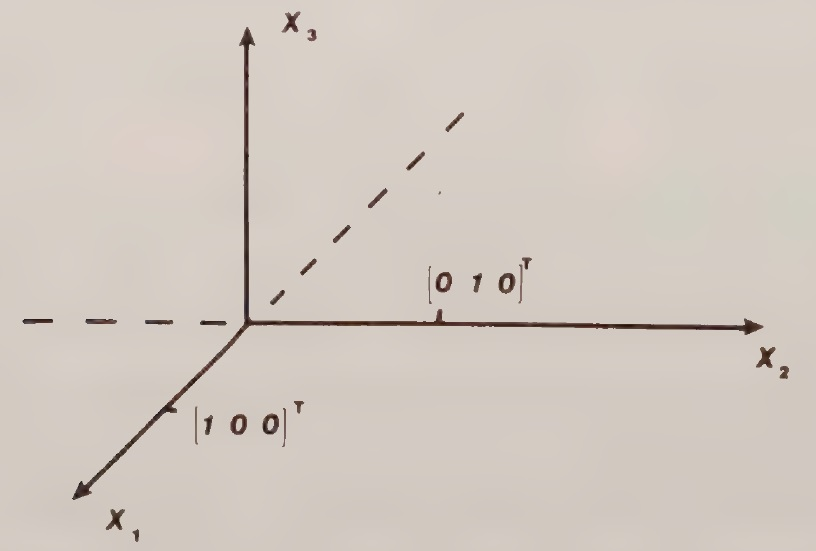
\includegraphics[width=\linewidth,height=0.61\textheight,keepaspectratio]{figures/mp-2026/p068-hulls-example.jpg}
    \end{column}
  \end{columns}
\end{frame}

% Source PDF page 069; convex-cone characterization corrected.
\begin{frame}{Hulls Characterize the Corresponding Closed Operations}
  For nonempty $S\subseteq\R^n$:
  \begin{itemize}
    \item $S\subseteq\Conv(S)\subseteq\Aff(S)\subseteq\Lin(S)$;
    \item $S\subseteq\Conv(S)\subseteq\Cone(S)\subseteq\Lin(S)$;
    \item $S$ is a subspace iff $S=\Lin(S)$;
    \item $S$ is affine iff $S=\Aff(S)$;
    \item $S$ is a convex cone iff $S=\Cone(S)$;
    \item $S$ is convex iff $S=\Conv(S)$.
  \end{itemize}
  Geometrically: affine sets contain full lines, convex cones contain nonnegative combinations, and convex sets contain line segments.
\end{frame}

% Source PDF page 070
\begin{frame}{An Affine Set Is a Translated Subspace}
  A nonempty set $S\subseteq\R^n$ is affine iff, for any $\vect{x}_0\in S$,
  \begin{equation*}
    S-\vect{x}_0=\{\vect{x}-\vect{x}_0:\vect{x}\in S\}
  \end{equation*}
  is a linear subspace.
  \begin{columns}[T,onlytextwidth]
    \begin{column}{0.47\textwidth}
      \begin{itemize}
        \item $S=\vect{x}_0+V$ for a subspace $V$;
        \item $\dim(S)=\dim(V)$;
        \item for a set $T$, $\dim(T)$ is defined as $\dim\Aff(T)$.
      \end{itemize}
    \end{column}
    \begin{column}{0.49\textwidth}
      \centering
      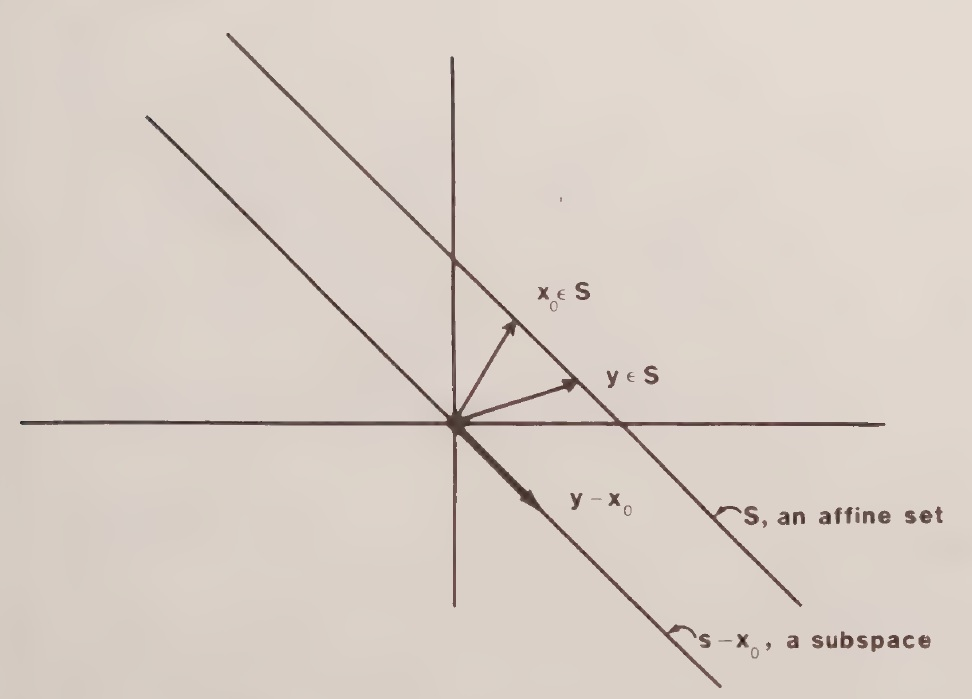
\includegraphics[width=\linewidth,height=0.42\textheight,keepaspectratio]{figures/mp-2026/p070-affine-translate.jpg}
    \end{column}
  \end{columns}
\end{frame}

\subsection{Hyperplanes, Polytopes, and Extreme Points}

% Source PDF page 071
\begin{frame}{A Hyperplane Separates Two Halfspaces}
  For $\vect{c}\ne\vect{0}$ and $\beta\in\R$:
  \begin{align*}
    \mathcal H(\vect{c},\beta)
      &=\{\vect{x}:\vect{c}^{\trans}\vect{x}=\beta\},\\
    \mathcal H^{+}(\vect{c},\beta)
      &=\{\vect{x}:\vect{c}^{\trans}\vect{x}\ge\beta\},\\
    \mathcal H^{-}(\vect{c},\beta)
      &=\{\vect{x}:\vect{c}^{\trans}\vect{x}\le\beta\}.
  \end{align*}
  \begin{center}
    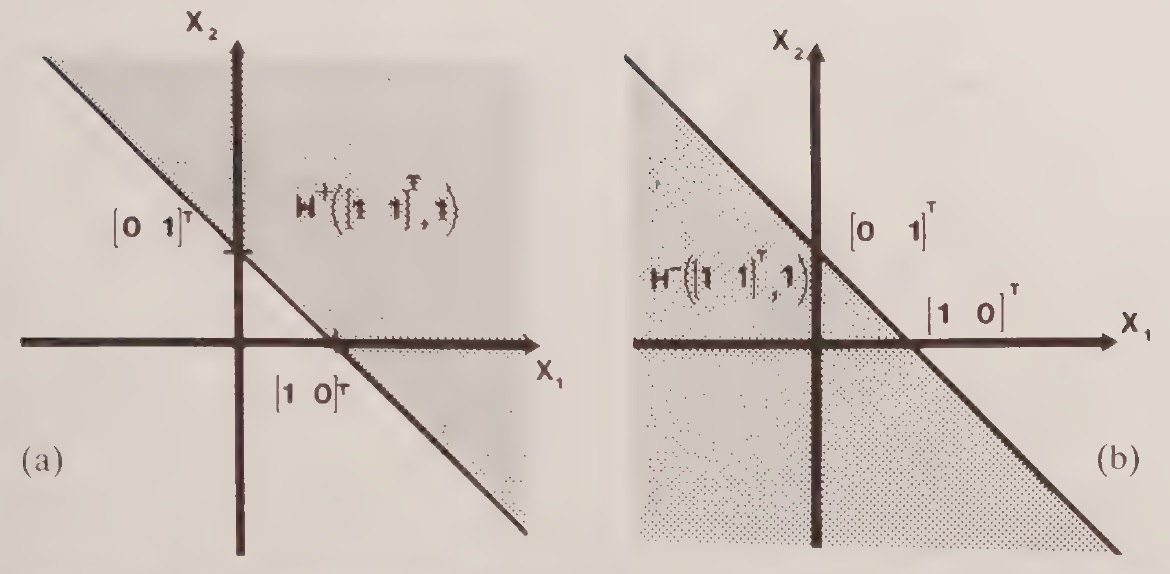
\includegraphics[width=0.48\linewidth,height=0.26\textheight,keepaspectratio]{figures/mp-2026/p071-hyperplane-halfspaces.jpg}
  \end{center}
\end{frame}

% Source PDF page 072
\begin{frame}{A Simplex Is the Basic Affinely Independent Polytope}
  \begin{columns}[T,onlytextwidth]
    \begin{column}{0.53\textwidth}
      \begin{itemize}
        \item A convex polytope is the convex hull of finitely many points:
          \begin{equation*}
            P=\Conv\{\vect{x}_1,\ldots,\vect{x}_k\}.
          \end{equation*}
        \item $\{\vect{x}_0,\ldots,\vect{x}_k\}$ is affinely independent iff $\{\vect{x}_1-\vect{x}_0,\ldots,\vect{x}_k-\vect{x}_0\}$ is linearly independent.
        \item A $k$-simplex is the convex hull of $k+1$ affinely independent points.
      \end{itemize}
    \end{column}
    \begin{column}{0.43\textwidth}
      \centering
      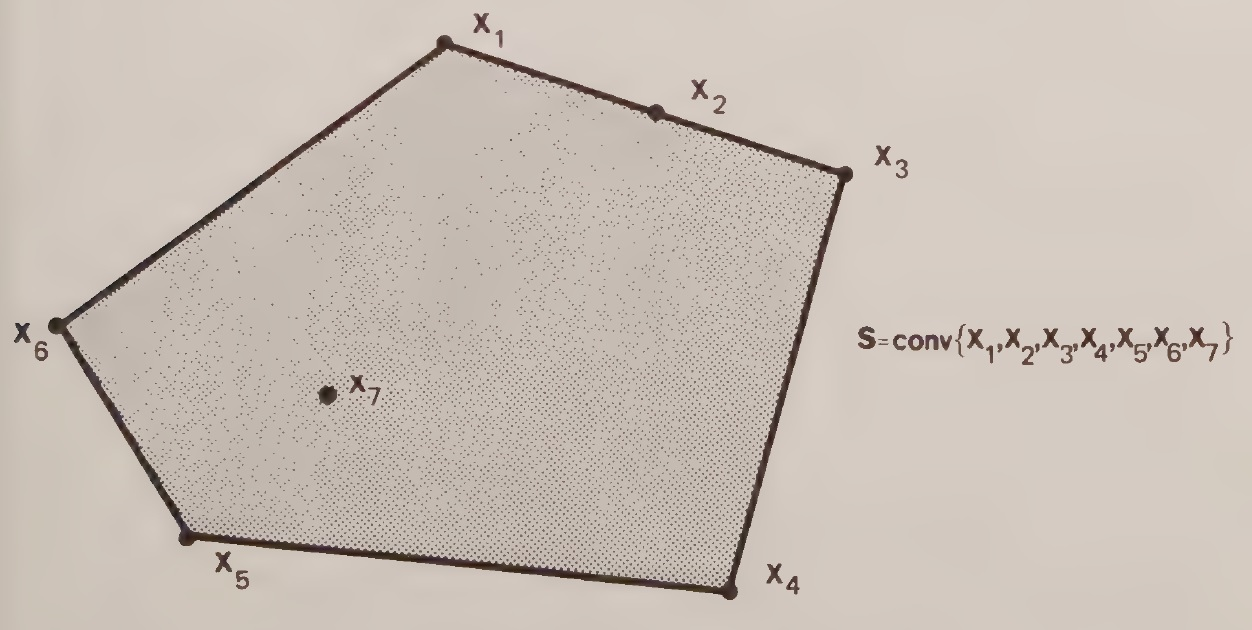
\includegraphics[width=\linewidth,height=0.55\textheight,keepaspectratio]{figures/mp-2026/p072-convex-polytope.jpg}
    \end{column}
  \end{columns}
\end{frame}

% Source PDF page 073
\begin{frame}{Segments, Triangles, and Tetrahedra Are Simplices}
  \centering
  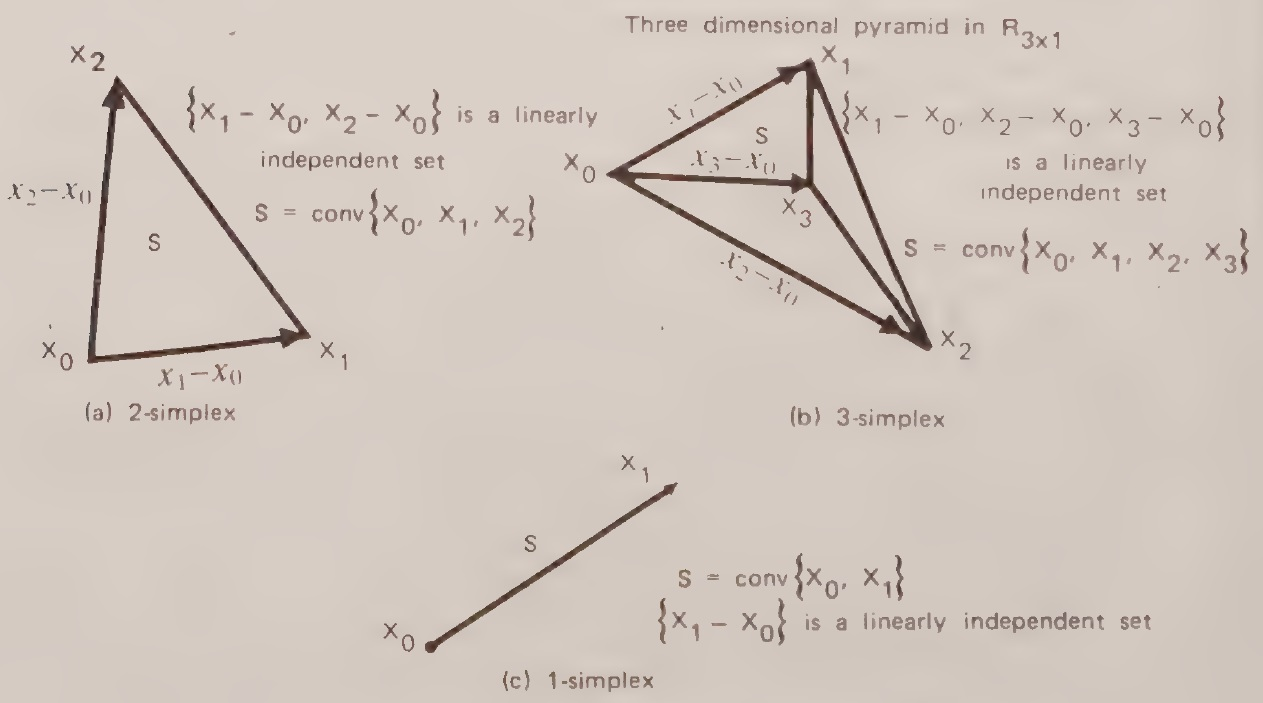
\includegraphics[width=0.78\linewidth,height=0.63\textheight,keepaspectratio]{figures/mp-2026/p073-simplex-examples.jpg}

  \vspace{0.3em}
  A 1-simplex is a segment, a 2-simplex is a triangle, and a 3-simplex is a tetrahedron.
\end{frame}

% Source PDF page 074
\begin{frame}{Extreme Points Cannot Be Written as Nontrivial Convex Mixtures}
  A point $\vect{z}\in S$, with $S$ convex, is extreme if
  \begin{equation*}
    \vect{z}=\alpha\vect{x}+(1-\alpha)\vect{y},
    \quad \vect{x},\vect{y}\in S,
    \quad0<\alpha<1
  \end{equation*}
  implies $\vect{x}=\vect{y}=\vect{z}$.
  \begin{columns}[T,onlytextwidth]
    \begin{column}{0.50\textwidth}
      \begin{itemize}
        \item Every vertex of a simplex is an extreme point.
        \item An extreme point is not in the relative interior of a segment joining two distinct points of $S$.
      \end{itemize}
    \end{column}
    \begin{column}{0.46\textwidth}
      \centering
      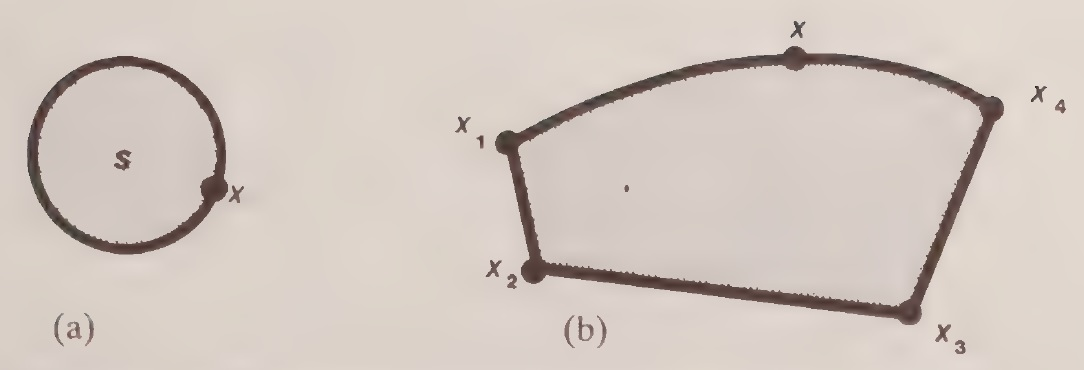
\includegraphics[width=\linewidth,height=0.34\textheight,keepaspectratio]{figures/mp-2026/p074-extreme-points.jpg}
    \end{column}
  \end{columns}
\end{frame}

\section{Linear Programming Geometry}
\subsection{Feasible Polyhedra}

% Source PDF page 075
\begin{frame}{A Linear Program Can Be Written Componentwise}
  \begin{equation*}
    \begin{aligned}
      \min_{\vect{x}}\quad
        &c_1x_1+\cdots+c_nx_n\\
      \text{subject to}\quad
        &a_{i1}x_1+\cdots+a_{in}x_n\le b_i,
          &&i=1,\ldots,m,\\
        &x_j\ge0,&&j=1,\ldots,n.
    \end{aligned}
  \end{equation*}
  Componentwise notation exposes the role of each variable and each constraint.
\end{frame}

% Source PDF page 076; feasible-set notation corrected.
\begin{frame}{Matrix Notation Reveals the Feasible Geometry}
  The same problem is
  \begin{equation*}
    \min_{\vect{x}}\ \vect{c}^{\trans}\vect{x}
    \quad\text{subject to}\quad
    A\vect{x}\le\vect{b},\quad\vect{x}\ge\vect{0}.
  \end{equation*}
  Since
  \begin{equation*}
    A\vect{x}=A^{(1)}x_1+\cdots+A^{(n)}x_n,
  \end{equation*}
  the feasible set is
  \begin{equation*}
    F=\{\vect{x}\in\R^n:A\vect{x}\le\vect{b},\ \vect{x}\ge\vect{0}\}.
  \end{equation*}
\end{frame}

% Source PDF page 077
\begin{frame}{The Feasible Set of a Linear Program Is Convex}
  Let $\vect{x}_1,\vect{x}_2\in F$ and $\alpha\in[0,1]$. For
  \begin{equation*}
    \vect{z}=\alpha\vect{x}_1+(1-\alpha)\vect{x}_2,
  \end{equation*}
  linearity gives
  \begin{equation*}
    A\vect{z}=\alpha A\vect{x}_1+(1-\alpha)A\vect{x}_2\le\vect{b},
    \qquad \vect{z}\ge\vect{0}.
  \end{equation*}
  Hence $\vect{z}\in F$.
  \begin{itemize}
    \item A polyhedron is an intersection of finitely many closed halfspaces.
    \item Every polytope is a bounded polyhedron.
    \item Every bounded polyhedron is a polytope; an unbounded polyhedron is not.
  \end{itemize}
\end{frame}

% Source PDF page 078
\begin{frame}{Boundedness Distinguishes Polytopes from General Polyhedra}
  \begin{columns}[T,onlytextwidth]
    \begin{column}{0.48\textwidth}
      \centering
      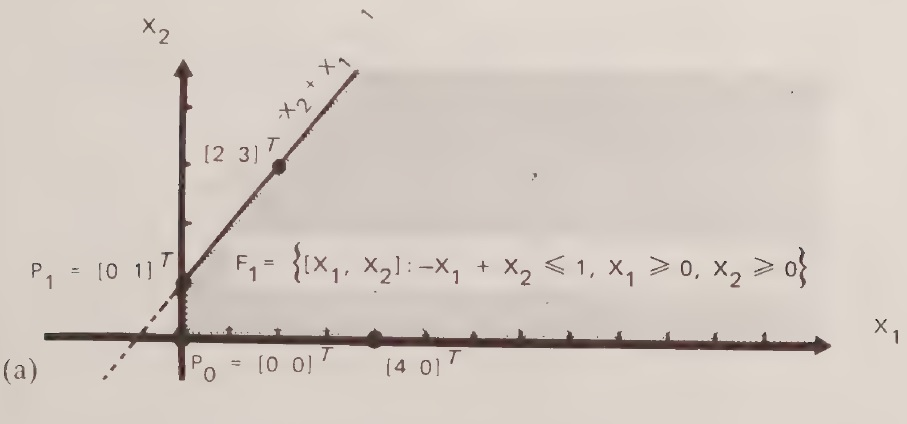
\includegraphics[width=\linewidth,height=0.48\textheight,keepaspectratio]{figures/mp-2026/p078-unbounded-polyhedron.jpg}

      \small Unbounded polyhedron: not a polytope.
    \end{column}
    \begin{column}{0.48\textwidth}
      \centering
      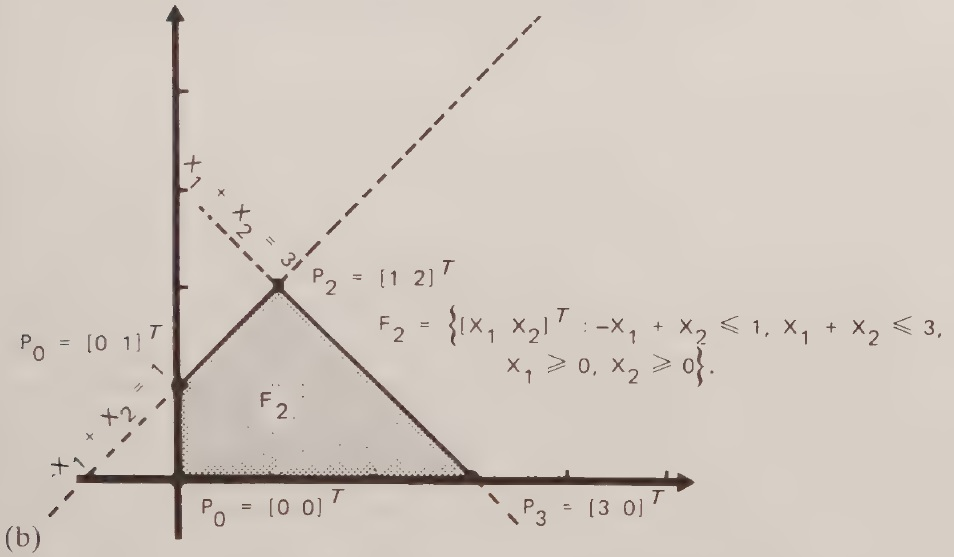
\includegraphics[width=\linewidth,height=0.48\textheight,keepaspectratio]{figures/mp-2026/p078-bounded-polytope.jpg}

      \small Bounded polyhedron: a polytope.
    \end{column}
  \end{columns}
\end{frame}

% Source PDF page 079; stated in standard Minkowski-Weyl form.
\begin{frame}{Minkowski-Weyl Gives a Finite Description of Every Polyhedron}
  \begin{block}{Finite generation theorem}
    A nonempty polyhedron $F\subseteq\R^n$ can be represented using finite sets of points $\{\vect{x}_1,\ldots,\vect{x}_d\}$ and rays $\{\vect{y}_1,\ldots,\vect{y}_{\ell}\}$:
    \begin{equation*}
      F=\Conv\{\vect{x}_1,\ldots,\vect{x}_d\}
        +\Cone\{\vect{y}_1,\ldots,\vect{y}_{\ell}\}.
    \end{equation*}
  \end{block}
  Equivalently,
  \begin{equation*}
    \vect{x}=\sum_{i=1}^{d}\alpha_i\vect{x}_i
      +\sum_{j=1}^{\ell}\beta_j\vect{y}_j,
    \quad \alpha_i,\beta_j\ge0,
    \quad\sum_{i=1}^{d}\alpha_i=1.
  \end{equation*}
\end{frame}

% Source PDF page 080
\begin{frame}{A Polyhedron Combines a Bounded Base with Recession Rays}
  \begin{columns}[T,onlytextwidth]
    \begin{column}{0.47\textwidth}
      For the illustrated set,
      \begin{equation*}
        F_2=\Conv\{\vect{p}_0,\vect{p}_1\}
          +\Cone\{\vect{v}_0,\vect{v}_1\}.
      \end{equation*}
      Thus every $\vect{x}\in F_2$ has the form
      \begin{equation*}
        \vect{x}=\alpha_0\vect{p}_0+\alpha_1\vect{p}_1
          +\beta_0\vect{v}_0+\beta_1\vect{v}_1,
      \end{equation*}
      where $\alpha_0+\alpha_1=1$ and all coefficients are nonnegative.
    \end{column}
    \begin{column}{0.49\textwidth}
      \centering
      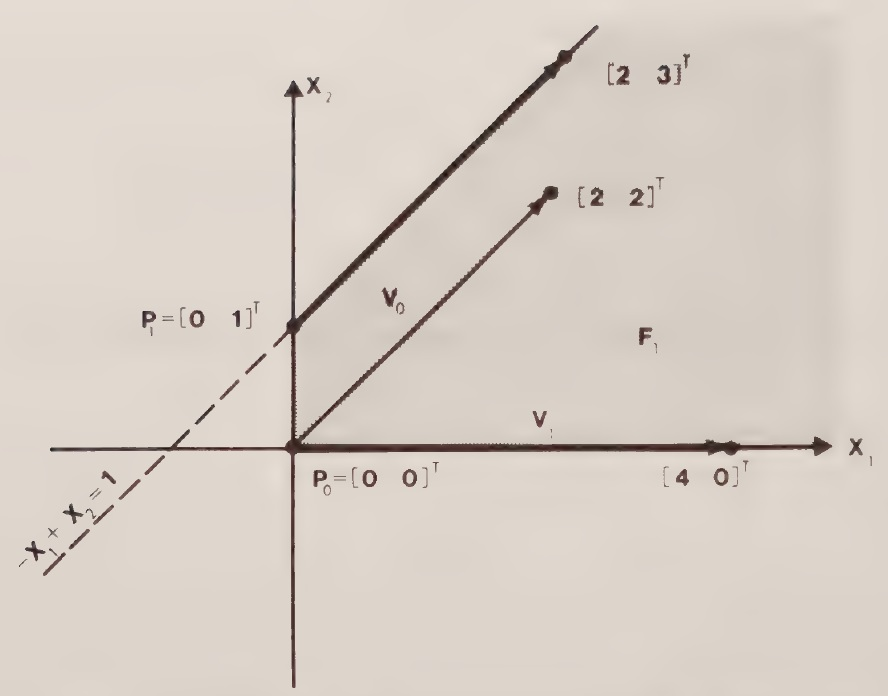
\includegraphics[width=\linewidth,height=0.58\textheight,keepaspectratio]{figures/mp-2026/p080-finite-basis-decomposition.jpg}
    \end{column}
  \end{columns}
\end{frame}

\end{document}
